%%%%%%%%%%%%%%%%%%%%%%%%%%%%%%%%%%%%%%%%%%%%%%%%%%%%%%%%%%%%%%%%%%%%%%%%%%%
%% This file is part of the book
%%
%% Algorithmic Graph Theory
%% http://code.google.com/p/graph-theory-algorithms-book/
%%
%% Copyright (C) 2009, 2010, 2011 Minh Van Nguyen <nguyenminh2@gmail.com>
%%
%% See the file COPYING for copying conditions.
%%%%%%%%%%%%%%%%%%%%%%%%%%%%%%%%%%%%%%%%%%%%%%%%%%%%%%%%%%%%%%%%%%%%%%%%%%%

\documentclass{article}

\usepackage{subfigure}
\usepackage{tikz}
\usetikzlibrary{external}
\usetikzlibrary{trees}
\tikzexternalize{sample-binary-heaps}

\begin{document}

\begin{figure}
\subfigure[]{
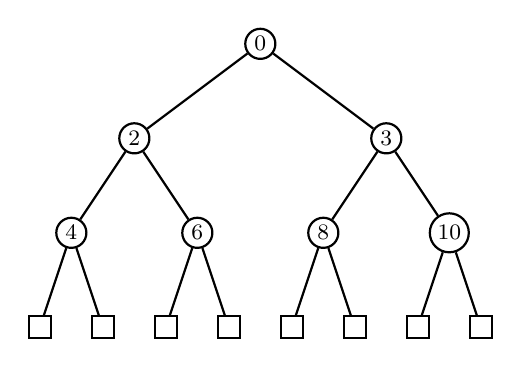
\begin{tikzpicture}
[-,thick,%
  every node/.style={shape=circle,inner sep=1.5pt,draw,thick},%
  scale=0.8]
\footnotesize
\node {$0$}
  [sibling distance=4cm]
  child {node {$2$}
    [sibling distance=2cm]
    child {node {$4$}
      [sibling distance=1cm]
      child {node[rectangle,inner sep=4pt,draw,thick] {}}
      child {node[rectangle,inner sep=4pt,draw,thick] {}}
    }
    child {node {$6$}
      [sibling distance=1cm]
      child {node[rectangle,inner sep=4pt,draw,thick] {}}
      child {node[rectangle,inner sep=4pt,draw,thick] {}}
    }
  }
  child {node {$3$}
    [sibling distance=2cm]
    child {node {$8$}
      [sibling distance=1cm]
      child {node[rectangle,inner sep=4pt,draw,thick] {}}
      child {node[rectangle,inner sep=4pt,draw,thick] {}}
    }
    child {node {$10$}
      [sibling distance=1cm]
      child {node[rectangle,inner sep=4pt,draw,thick] {}}
      child {node[rectangle,inner sep=4pt,draw,thick] {}}
    }
  };
\end{tikzpicture}
}
%%
%%
\subfigure[]{
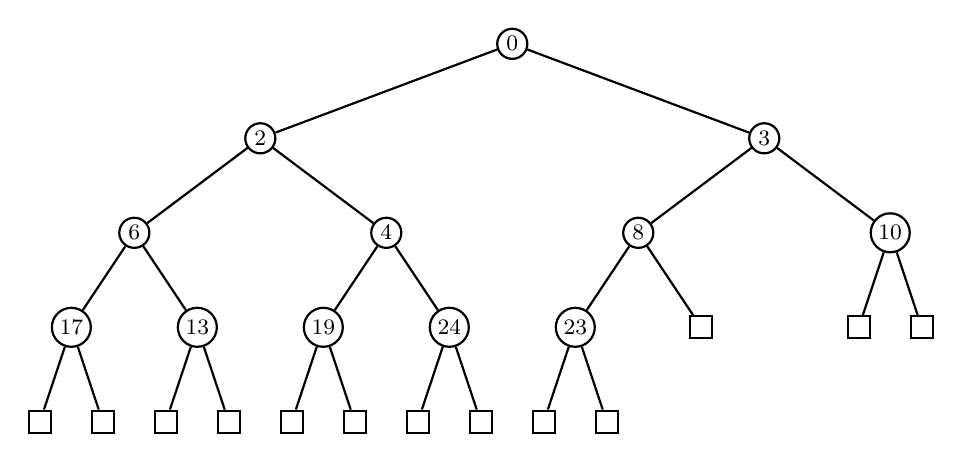
\begin{tikzpicture}
[-,thick,%
  every node/.style={shape=circle,inner sep=1.5pt,draw,thick},%
  scale=0.8]
\footnotesize
\node {$0$}
  [sibling distance=8cm]
  child {node {$2$}
    [sibling distance=4cm]
    child {node {$6$}
      [sibling distance=2cm]
      child {node {$17$}
        [sibling distance=1cm]
        child {node[rectangle,inner sep=4pt,draw,thick] {}}
        child {node[rectangle,inner sep=4pt,draw,thick] {}}
      }
      child {node {$13$}
        [sibling distance=1cm]
        child {node[rectangle,inner sep=4pt,draw,thick] {}}
        child {node[rectangle,inner sep=4pt,draw,thick] {}}
      }
    }
    child {node {$4$}
      [sibling distance=2cm]
      child {node {$19$}
        [sibling distance=1cm]
        child {node[rectangle,inner sep=4pt,draw,thick] {}}
        child {node[rectangle,inner sep=4pt,draw,thick] {}}
      }
      child {node {$24$}
        [sibling distance=1cm]
        child {node[rectangle,inner sep=4pt,draw,thick] {}}
        child {node[rectangle,inner sep=4pt,draw,thick] {}}
      }
    }
  }
  child {node {$3$}
    [sibling distance=4cm]
    child {node {$8$}
      [sibling distance=2cm]
      child {node {$23$}
        [sibling distance=1cm]
        child {node[rectangle,inner sep=4pt,draw,thick] {}}
        child {node[rectangle,inner sep=4pt,draw,thick] {}}
      }
      child {node[rectangle,inner sep=4pt,draw,thick] {}}
    }
    child {node {$10$}
      [sibling distance=1cm]
      child {node[rectangle,inner sep=4pt,draw,thick] {}}
      child {node[rectangle,inner sep=4pt,draw,thick] {}}
    }
  };
\end{tikzpicture}
}
%%
%%
\subfigure[]{
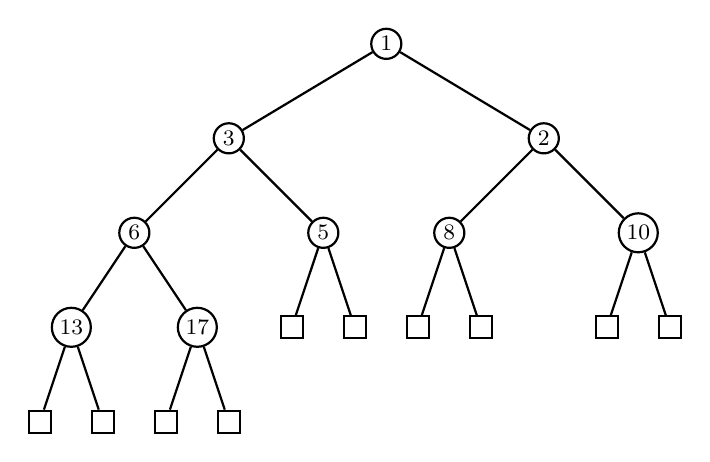
\begin{tikzpicture}
[-,thick,%
  every node/.style={shape=circle,inner sep=1.5pt,draw,thick},%
  scale=0.8]
\footnotesize
\node {$1$}
  [sibling distance=5cm]
  child {node {$3$}
    [sibling distance=3cm]
    child {node {$6$}
      [sibling distance=2cm]
      child {node {$13$}
        [sibling distance=1cm]
        child {node[rectangle,inner sep=4pt,draw,thick] {}}
        child {node[rectangle,inner sep=4pt,draw,thick] {}}
      }
      child {node {$17$}
        [sibling distance=1cm]
        child {node[rectangle,inner sep=4pt,draw,thick] {}}
        child {node[rectangle,inner sep=4pt,draw,thick] {}}
      }
    }
    child {node {$5$}
      [sibling distance=1cm]
      child {node[rectangle,inner sep=4pt,draw,thick] {}}
      child {node[rectangle,inner sep=4pt,draw,thick] {}}
    }
  }
  child {node {$2$}
    [sibling distance=3cm]
    child {node {$8$}
      [sibling distance=1cm]
      child {node[rectangle,inner sep=4pt,draw,thick] {}}
      child {node[rectangle,inner sep=4pt,draw,thick] {}}
    }
    child {node {$10$}
      [sibling distance=1cm]
      child {node[rectangle,inner sep=4pt,draw,thick] {}}
      child {node[rectangle,inner sep=4pt,draw,thick] {}}
    }
  };
\end{tikzpicture}
}
\end{figure}

\end{document}
